%% CacheFlow: Caching What the Model Produces, Not Just What It Reads
%% Compile with: pdflatex whitepaper.tex  (run twice for cross-references)
\documentclass[10pt]{article}

% --- Encoding & fonts ---------------------------------------------------
\usepackage[T1]{fontenc}
\usepackage[utf8]{inputenc}
\usepackage{lmodern}
\usepackage{microtype}

% --- Layout -------------------------------------------------------------
\usepackage[letterpaper,margin=1in]{geometry}
\usepackage{titlesec}
\usepackage{abstract}
\usepackage{enumitem}
\setlist{noitemsep,topsep=3pt,leftmargin=1.4em}

% --- Float placement -----------------------------------------------------
% Defaults are conservative and push large table*/figure floats (esp. the
% full-width results tables) several pages past their reference point,
% forcing the reader to jump ahead then back. Loosen the thresholds so
% floats place near where they're cited instead of drifting to a float page.
\renewcommand{\topfraction}{0.9}
\renewcommand{\dbltopfraction}{0.9}
\renewcommand{\textfraction}{0.07}
\renewcommand{\floatpagefraction}{0.7}
\renewcommand{\dblfloatpagefraction}{0.7}
\setcounter{topnumber}{3}
\setcounter{dbltopnumber}{3}
\setcounter{totalnumber}{4}

% --- Math, tables, code -------------------------------------------------
\usepackage{amsmath,amssymb}
\usepackage{booktabs}
\usepackage{array}
\usepackage{multirow}
\usepackage{siunitx}
\sisetup{group-separator={,},group-minimum-digits=4,detect-weight=true}
\DeclareSIUnit{\flop}{FLOP}
\DeclareSIUnit{\tokens}{tokens}
\usepackage{xcolor}
\definecolor{cfblue}{RGB}{20,70,140}
\definecolor{cfgray}{RGB}{95,95,95}
\definecolor{codebg}{RGB}{246,246,248}
\usepackage{listings}
\lstset{
  basicstyle=\ttfamily\footnotesize,
  backgroundcolor=\color{codebg},
  breaklines=true,
  columns=fullflexible,
  keepspaces=true,
  frame=single,
  framesep=4pt,
  rulecolor=\color{cfgray!40},
  aboveskip=6pt,belowskip=4pt,
  xleftmargin=2pt,xrightmargin=2pt,
}

% --- Algorithms & diagrams ---------------------------------------------
\usepackage[ruled,vlined,linesnumbered]{algorithm2e}
\usepackage{tikz}
\usetikzlibrary{arrows.meta,positioning,fit,backgrounds,calc,shapes.geometric}
\tikzset{
  box/.style={draw=cfgray!60,rounded corners=2pt,align=center,inner sep=4pt,font=\scriptsize,fill=white},
  store/.style={draw=cfblue!70,rounded corners=2pt,align=center,inner sep=4pt,font=\scriptsize,fill=cfblue!6},
  flow/.style={-{Latex[length=2mm]},draw=cfgray!80,thick},
}

% --- References ---------------------------------------------------------
\usepackage[colorlinks=true,allcolors=cfblue,breaklinks=true]{hyperref}
\usepackage{cleveref}

% --- Section styling ----------------------------------------------------
\titleformat{\section}{\normalfont\large\bfseries\color{cfblue}}{\thesection}{0.6em}{}
\titleformat{\subsection}{\normalfont\normalsize\bfseries}{\thesubsection}{0.6em}{}
\titlespacing*{\section}{0pt}{10pt}{4pt}
\titlespacing*{\subsection}{0pt}{7pt}{2pt}

% --- Title metadata -----------------------------------------------------
\title{\vspace{-2.5em}\textbf{\color{cfblue}CacheFlow}: Caching Generated Reasoning,\\Not Just the Prompt, for Persistent-Memory Coding Agents}

\author{%
  Agastya Choudhary\\
  \normalsize\texttt{agastya.r.choudhary@gmail.com}
}
\date{\normalsize July 8, 2026}

% ======================================================================
\begin{document}
\maketitle
\begin{abstract}
\noindent
Coding agents pay for the same computation twice. On \emph{self-hosted} models
the prompt prefix---a system prompt plus tens of thousands of tokens of
codebase context---is re-evaluated on every invocation even though its
attention (KV) state is deterministic and reusable. On \emph{cloud-hosted}
models the situation is worse: provider prompt caching amortizes the stable
prefix, but \emph{extended-thinking tokens}---the reasoning a model generates
before answering---are produced fresh on every call and cannot be cached at
all, because they are generated output, not cached input. In multi-agent and
multi-step workflows, independent agents re-reason about the same problem and
re-read the same files, paying full reasoning cost each time.
We present \textsc{CacheFlow}, a persistent-memory layer that addresses both
costs with mechanisms matched to what each deployment actually exposes. For
self-hosted \texttt{llama.cpp} models, \textsc{CacheFlow} serializes and
restores per-sequence KV state, turning a multi-second cold prefill into a
sub-second warm restore. For cloud models, where no internal state is
retrievable, it instead caches the model's \emph{outputs}: a content-addressed
\emph{thinking-block store} with confidence-gated semantic reuse. Across eight
real-world Python corpora we measure a cold prime replaced by a
$\sim$\SI{300}{\milli\second} warm restore, cumulatively
$\sim$\SI{246}{\second} of wall-clock prefill and $\sim$\SI{1500}{\tera\flop}
of compute avoided on the self-hosted path, and exact, API-reported reductions
of up to 100\% of a turn's reasoning tokens on the cloud path, with all savings
computed from real token counts rather than estimated from text length.
\end{abstract}
\vspace{1em}

% ======================================================================
\section{Introduction}
\label{sec:intro}

Large-language-model coding agents are increasingly deployed as
\emph{long-lived, multi-step, multi-agent} systems: a planner delegates to an
implementer, a reviewer inspects the diff, a tester exercises the change, and
each of these may run dozens of tool-calling iterations. Every one of these
invocations begins by presenting the model with a large, mostly-stable context
(a system prompt plus a substantial slice of the codebase) and then asks the
model to reason toward an action.

Two distinct, recurring costs arise from this pattern, and---critically---they
have \emph{different} solutions depending on whether the model is self-hosted or
cloud-hosted:

\begin{enumerate}
  \item \textbf{Prefix re-evaluation (self-hosted).} A self-hosted model
  exposes its own attention/KV state. Yet most serving stacks discard that
  state between calls and re-run the full prefill over the stable prefix,
  spending seconds of wall-clock time and hundreds of TFLOPs re-deriving a
  state that is deterministic given the same tokens and model.
  \item \textbf{Reasoning regeneration (cloud-hosted).} A cloud API never
  exposes internal state; there is no \texttt{llama\_state\_seq\_get\_data}
  equivalent to call. Provider-side prompt caching~\cite{anthropic-caching}
  amortizes the \emph{input} prefix, but \emph{extended-thinking} tokens are
  \emph{generated output}. They are recomputed on every call and, once a
  provider's short cache TTL lapses, cannot be shared even between two agents
  solving the identical problem minutes apart.
\end{enumerate}

The central observation of this paper is that these are two faces of the same
waste---\emph{recomputing a deterministic function of the same inputs}---but
that they must be attacked at different layers because cloud and self-hosted
deployments expose different surfaces. Where the model's internals are
reachable, cache the \emph{internals} (KV state). Where they are not, cache the
model's \emph{outputs} (reasoning traces and derived understanding).

\textsc{CacheFlow} implements both. It began as a KV-cache restoration system
for self-hosted \texttt{llama.cpp} models (\Cref{sec:kv}) and was extended with
an output-caching layer for cloud models (\Cref{sec:cloud}). The two subsystems
share design philosophy---content-hash-based staleness, snapshot/GC lifecycle,
exact rather than estimated metrics---but are fully independent in storage and
invalidation.

\paragraph{Contributions.}
\begin{itemize}
  \item A persistent per-sequence KV-cache snapshot/restore system for
  self-hosted models that skips the redundant warm-path save and forces a safe
  re-prime on codebase or model change (\Cref{sec:kv}).
  \item An output-caching layer for cloud models: a content-addressed,
  confidence-gated \emph{thinking-block store} (\Cref{sec:cloud}).
  \item A discipline of \emph{exact} token accounting: every savings figure is
  a real, provider-reported token count, never estimated from character length
  (\Cref{sec:metrics}).
  \item An evaluation across eight real-world Python corpora quantifying both
  paths, including honest reporting of zero-hit cases (\Cref{sec:eval}).
\end{itemize}

% ======================================================================
\section{Background and Motivation}
\label{sec:background}

\subsection{The Prefill Tax on Self-Hosted Models}
Transformer inference proceeds in two phases: a compute-bound \emph{prefill}
that populates the KV cache for every prompt token in parallel, and a
bandwidth-bound \emph{decode} that emits output tokens one at a time. For a
coding agent whose prompt is dominated by a fixed system prompt and codebase
slice, prefill is pure overhead after the first call: the KV state for those
tokens is identical across invocations of the same model. A multi-thousand-token
codebase prefill on an 8B model costs on the order of tens of seconds of
wall-clock time and hundreds of TFLOPs in our measurements (\Cref{sec:eval}:
e.g.\ a cold prime of $\sim$\SI{20}{\second} on the \texttt{requests} corpus),
all of it re-derivable from disk in milliseconds if the state is persisted.

\subsection{The Reasoning Tax on Cloud Models}
Extended thinking lets a model emit an internal reasoning trace before its final
answer, materially improving performance on hard tasks. But this trace is
\emph{output}: it is billed as output tokens and regenerated on every call.
Consider a single agent running a 20-step tool-use loop at $\sim$\num{5000}
thinking tokens per step: \num{100000} reasoning tokens, none of which any
provider cache can eliminate. In a multi-agent workflow the same reasoning is
paid two or three times as each agent independently re-derives it. And because
provider caches expire on the order of minutes, an agent that starts even
slightly after another gets no benefit from the first agent's work.

\subsection{Why Existing Techniques Are Insufficient}
Provider prompt caching~\cite{anthropic-caching} and prefix-reuse systems such
as PromptCache~\cite{promptcache} and PagedAttention~\cite{pagedattention}
target the \emph{input} prefix; they do not touch generated reasoning.
Context-compaction and summarization reduce message bloat but do not stop each
agent from thinking independently. Retrieval-augmented
generation~\cite{rag} injects relevant documents but does not cache the
\emph{conclusions} an agent reaches. \textsc{CacheFlow}'s cloud path is
complementary to all of these: it caches the reasoning and the derived
understanding themselves.

% ======================================================================
\section{Problem Formulation}
\label{sec:problem}

We now make the two costs of \Cref{sec:intro} precise and derive the condition
under which caching is profitable. \Cref{tab:notation} fixes notation.

\begin{table}[t]
\centering
\caption{Notation.}
\label{tab:notation}
\footnotesize
\begin{tabular}{@{}l>{\raggedright\arraybackslash}p{0.70\columnwidth}@{}}
\toprule
\textbf{Symbol} & \textbf{Meaning} \\
\midrule
$P$ & length (tokens) of the stable prefix (system prompt $+$ code) \\
$s$ & length of the per-call task suffix, $s \ll P$ \\
$N$ & number of invocations sharing the same prefix/problem \\
$c_{\text{pre}}$ & cost to prefill one token (compute or wall-clock) \\
$c_{\text{res}}$ & cost to restore a KV snapshot from disk \\
$T_r$ & extended-thinking tokens generated on a cold reasoning turn \\
$T_v$ & tokens spent validating a borderline cached block \\
$\sigma(\cdot)$ & similarity score of a candidate cached artifact \\
$h$ & content hash; $h_w$ at write time, $h_r$ at read time \\
$p$ & empirical reuse (cache-hit) rate over the $N$ calls \\
$\theta_u,\theta_v$ & use-directly and validate confidence thresholds \\
\bottomrule
\end{tabular}
\end{table}

\subsection{Self-Hosted: the Prefill Recurrence}
Without persistence, every one of the $N$ calls re-prefills the whole prefix,
so total prefill cost is
\begin{equation}
C_{\text{base}} = N\,(P+s)\,c_{\text{pre}}.
\label{eq:base}
\end{equation}
With snapshot persistence the first call primes ($P$ tokens) and each subsequent
call restores the snapshot and prefills only its suffix:
\begin{equation}
C_{\text{cf}} = \underbrace{P\,c_{\text{pre}}}_{\text{one cold prime}}
   + (N\!-\!1)\big(c_{\text{res}} + s\,c_{\text{pre}}\big).
\label{eq:cf}
\end{equation}
Since $c_{\text{res}}\!\approx\!0$ relative to $P\,c_{\text{pre}}$ and
$s\ll P$, the per-warm-call saving approaches $P\,c_{\text{pre}}$ and the
speedup grows with prefix size:
\begin{equation}
\frac{C_{\text{base}}}{C_{\text{cf}}}
   \;\xrightarrow[\;s,\,c_{\text{res}}\to 0\;]{}\;
   \frac{N(P+s)}{P} \;\approx\; N .
\label{eq:speedup}
\end{equation}
The compute form of $c_{\text{pre}}$ is not constant in $P$: a decoder layer's
attention contributes a term quadratic in sequence length. For a model of $\Pi$
parameters, $L$ layers, and hidden width $d$, the FLOPs avoided by skipping a
prefill of $n$ tokens is
\begin{equation}
\mathcal{F}(n) \;=\; \underbrace{2\,\Pi\,n}_{\text{dense (linear)}}
   \;+\; \underbrace{2\,L\,d\,n^{2}}_{\text{self-attention (quadratic)}} .
\label{eq:flops}
\end{equation}
We evaluate \Cref{eq:flops} with $\Pi$, $L$, $d$ read exactly from the loaded
GGUF (\Cref{sec:metrics}), never estimated from a model-name size tag.

\subsection{Cloud: Expected Reasoning Cost Under Reuse}
On the cloud path there is no $c_{\text{res}}$ to exploit; the recurring cost is
the reasoning $T_r$ regenerated per call. Let $p$ be the fraction of calls that
find a usable cached block. A cold call costs $T_r$; a validated reuse costs only
$T_v$ (the confirmation call, $T_v \ll T_r$); an exact/high-confidence reuse
costs $0$. Modelling the hit population as a fraction $\alpha$ of exact or
high-confidence hits and $1-\alpha$ validated hits, the expected per-call
reasoning cost is
\begin{equation}
\mathbb{E}[T] \;=\; (1-p)\,T_r \;+\; p\big[(1-\alpha)\,T_v\big],
\label{eq:expected}
\end{equation}
and the fractional reasoning saving is
\begin{equation}
\eta \;=\; 1 - \frac{\mathbb{E}[T]}{T_r}
     \;=\; p\Big(1 - (1-\alpha)\tfrac{T_v}{T_r}\Big).
\label{eq:eta}
\end{equation}
\Cref{eq:eta} makes the design tension explicit: savings rise with hit rate $p$,
but a reused block that is \emph{wrong} corrupts the downstream call, so $p$ must
be earned conservatively rather than maximised (\Cref{sec:thinking}).

\subsection{The Reuse Decision}
Retrieval returns the best candidate and a calibrated confidence
$\kappa\!\in\![0,1]$; the action is a thresholded decision
\begin{equation}
a(\kappa)=
\begin{cases}
\textsc{use\_directly} & \kappa \ge \theta_u,\\
\textsc{validate} & \theta_v \le \kappa < \theta_u,\\
\textsc{re\_think} & \kappa < \theta_v.
\end{cases}
\label{eq:decision}
\end{equation}
Confidence combines raw similarity with an age penalty; for a block written
$t$ days ago,
\begin{equation}
\kappa \;=\; \sigma(\cdot)\cdot e^{-\lambda t}, \qquad \lambda = 0.1,
\label{eq:agedecay}
\end{equation}
a $\sim$7-day half-life reflecting that older reasoning was computed against a
codebase that has since drifted. When the pool holds $\ge\!8$ blocks we replace
the absolute $\sigma$ with a scale-invariant background $z$-score
\begin{equation}
z \;=\; \frac{\sigma^\star - \mu_\sigma}{\varsigma_\sigma},
\label{eq:zscore}
\end{equation}
where $\sigma^\star$ is the top candidate's similarity and $\mu_\sigma,
\varsigma_\sigma$ are the mean and standard deviation of the query's similarity
to the rest of the pool---measuring how far the best hit \emph{stands out},
which transfers across domains where the absolute scale of $\sigma$ does not.

\subsection{Staleness as a Hash Predicate}
Both subsystems replace explicit invalidation with a write-time/read-time hash
comparison. An artifact is served iff
\begin{equation}
\textsc{valid} \iff h_r = h_w,
\label{eq:stale}
\end{equation}
so any edit to the underlying prefix, file region, or model silently changes
$h_r$ and suppresses the stale artifact with no separate expiry path.

% ======================================================================
\section{System Overview}
\label{sec:overview}

\textsc{CacheFlow} is a command-line tool (\texttt{cf}) and a set of libraries
packaged as a single Python distribution. It comprises two independent
subsystems joined by a shared philosophy but no shared state:

\begin{description}[leftmargin=1.1em,style=nextline]
  \item[Self-hosted KV engine] Serializes and restores per-sequence attention
  state for local \texttt{llama.cpp} models (\Cref{sec:kv}).
  \item[Cloud output cache] A SQLite-backed pool, \texttt{ThinkingStore}, that
  caches generated reasoning for cloud-hosted agents (\Cref{sec:cloud}).
\end{description}

Both subsystems detect staleness the same way: a content hash computed at
\emph{write} time is compared at \emph{read} time (\Cref{eq:stale}), so a
changed codebase or model silently invalidates the cached artifact with
no explicit expiry logic. They store to distinct SQLite databases
(\texttt{.cacheflow/agents.db}, \texttt{thinking.db}) and
share no foreign keys: a KV-snapshot restore and a thinking-block hit are
unrelated events that can each occur independently (\Cref{fig:arch}).

\begin{figure}[t]
\centering
\resizebox{\columnwidth}{!}{%
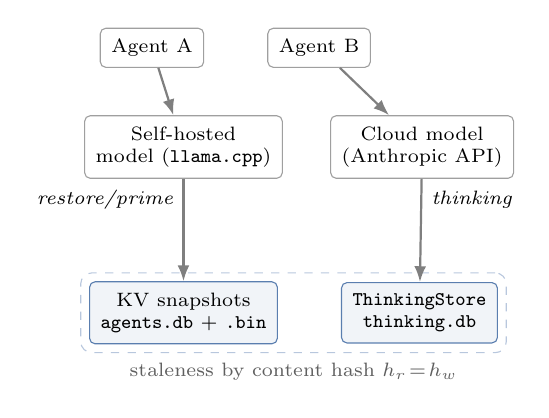
\begin{tikzpicture}[node distance=3.2mm]
\node[box] (agentA) {Agent A};
\node[box,right=8mm of agentA] (agentB) {Agent B};
\node[box,below=6mm of agentA,xshift=4mm] (self) {Self-hosted\\model (\texttt{llama.cpp})};
\node[box,right=6mm of self] (cloud) {Cloud model\\(Anthropic API)};
% stores
\node[store,below=13mm of self] (kv) {KV snapshots\\\texttt{agents.db} $+$ \texttt{.bin}};
\node[store,right=8mm of kv] (think) {\texttt{ThinkingStore}\\\texttt{thinking.db}};
% flows
\draw[flow] (agentA) -- (self);
\draw[flow] (agentB) -- (cloud);
\draw[flow] (self) -- node[pos=0.2,left,font=\scriptsize\itshape]{restore/prime} (kv);
\draw[flow] (cloud) -- node[pos=0.2,right,font=\scriptsize\itshape]{thinking} (think);
\begin{scope}[on background layer]
\node[draw=cfblue!30,dashed,rounded corners,fit=(kv)(think),inner sep=3pt,label={[font=\scriptsize\color{cfgray}]below:staleness by content hash $h_r\!=\!h_w$}] {};
\end{scope}
\end{tikzpicture}}
\caption{\textsc{CacheFlow}'s two independent subsystems. Where model internals
are reachable (self-hosted), it caches KV state; where they are not (cloud), it
caches generated \emph{reasoning}. No store shares keys with another.}
\label{fig:arch}
\end{figure}

% ======================================================================
\section{The Self-Hosted KV-Cache Engine}
\label{sec:kv}

\subsection{Core Flow: Restore/Prime $\rightarrow$ Save $\rightarrow$ Complete $\rightarrow$ Record}
Each agent maintains a HEAD pointer to at most one KV snapshot. A session
proceeds as:
\begin{enumerate}
  \item \textbf{Restore or Prime.} The agent computes
  \texttt{stable\_context} (system prompt $+$ codebase text) and its hash. If the
  agent's HEAD snapshot's \texttt{stable\_context\_hash} still matches, the
  snapshot is restored (\emph{warm path}). Otherwise the prefix is fed to the
  model to populate the KV cache (\emph{cold prime}).
  \item \textbf{Save.} On the prime path \emph{only}, the KV cache is serialized
  to disk. On the warm path this is skipped: the HEAD snapshot on disk is already
  byte-identical.
  \item \textbf{Complete.} The model generates using prefix matching---cached
  tokens plus the short ($\sim$5--50 token) task suffix.
  \item \textbf{Record.} The agent's HEAD and token/time metrics are updated in
  SQLite; savings are computed against the cold-prime baseline via
  \Cref{eq:base,eq:cf}.
\end{enumerate}

\begin{algorithm}[t]
\footnotesize
\DontPrintSemicolon
\caption{Restore-or-Prime session (self-hosted)}
\label{alg:restore}
\KwIn{agent $A$, stable context $X$, active model $M$}
$h_r \leftarrow \textsc{hash}(X)$\;
\uIf{$A.\text{head} \ne \varnothing \,\wedge\, A.\text{head}.h_w = h_r \,\wedge\, A.\text{head}.model = M$}{
  $\text{kv} \leftarrow \textsc{RestoreSnapshot}(A.\text{head})$ \tcp*{warm, $O(c_{\text{res}})$; save skipped}
}
\Else{
  $\text{kv} \leftarrow \textsc{Prefill}(X)$ \tcp*{cold: $O(P\,c_{\text{pre}})$}
  $\text{snap} \leftarrow \textsc{SerializeSeq}(\text{kv})$\;
  \textsc{WriteSnapshot}(\text{snap}); \quad $A.\text{head} \leftarrow \text{snap}$ \tcp*{write before HEAD update}
}
$y \leftarrow \textsc{Complete}(\text{kv}, \text{suffix})$\;
\textsc{RecordMetrics}(A);\ \Return $y$\;
\end{algorithm}

\Cref{alg:restore} makes the two safety invariants explicit: the warm branch is
taken only when \emph{both} the content hash and the model match (a snapshot is
raw KV bytes tied to one tokenizer/vocabulary), and the snapshot is written
\emph{before} HEAD is advanced, so a crash leaves $A$ on its previous valid
snapshot.

\subsection{Per-Sequence Snapshots (Format v4)}
Rather than serialize the full \texttt{n\_ctx} buffer, \textsc{CacheFlow} saves
only the live KV for the sequence via \texttt{llama\_state\_seq\_get\_data},
yielding compact snapshots ($\sim$\SI{8}{\mega\byte} of in-memory slot state per
idle agent). Because a snapshot is raw KV bytes tied to one model's tokenizer,
vocabulary, and hidden dimensions, a \texttt{model\_changed} guard in
\texttt{AgentSession} forces a re-prime (never a restore) whenever the active
model differs from the one that produced the snapshot.

\subsection{Concurrency, Consolidation, and GC}
A \texttt{SlotPool} manages up to eight concurrent KV slots with a
\texttt{SlotLease} context manager and LRU eviction that never evicts an
actively-running agent. Past 70\% of the context window, a background
\texttt{Compressor} restores HEAD, asks the model for a $\leq$\num{500}-token
knowledge summary, and folds it into the next session's stable prefix. A
\texttt{SnapshotGC} reaps snapshot files unreferenced by any agent's HEAD, plus
crash orphans; the write-snapshot-then-update-HEAD ordering guarantees a crash
leaves the agent on its previous valid snapshot.

\subsection{In-Process Execution}
The model runs in-process via \texttt{llama-cpp-python} rather than behind an
HTTP shim. On macOS an HTTP transport throttles decode by roughly
$10\times$; in-process execution avoids that path. Decode remains
bandwidth-bound at $\sim$\SI{5}{\tokens\per\second}, so the engine optimizes the
compute-bound prefill (\texttt{n\_batch}=\texttt{n\_ubatch}=\num{2048}) where
caching pays off, and a single global model instance (\texttt{get\_global\_engine})
is shared across all agents.

The prefill batch width is a deliberate choice. \texttt{llama.cpp} decodes a
prompt in chunks of \texttt{n\_batch} tokens; the default 512 forces a
multi-thousand-token codebase prefix through many sequential chunks. Raising
\texttt{n\_batch}=\texttt{n\_ubatch} to \num{2048} lets the same prefix populate
in a quarter as many passes, and the engine enables FlashAttention so that a
stable context spanning several batch chunks is attended to in a single fused
kernel with $O(d)$ rather than $O(n)$ intermediate memory per token---a
prerequisite for priming real-codebase contexts that exceed one batch width. A
one-time \texttt{atexit} teardown then frees the inference model and the
vocabulary-only tokenizer model (\Cref{sec:metrics}) in a fixed order, since
both hold buffers in the same \texttt{ggml} Metal device manager and must be
released deterministically rather than at interpreter-shutdown GC order.

\subsection{Per-Model Instruction Templating}
\label{sec:templates}
A KV snapshot is only reusable if every session wraps its turns in the byte-exact
token markers the model was trained on; a prefix that drifts by a single control
token no longer matches the cached KV. \textsc{CacheFlow} therefore selects an
instruction template per model rather than hard-coding one family. A
\texttt{ChatTemplate} record fixes the system/user wrappers, the assistant
open/close markers, and the generation stop token for each of five families
(\textsc{ChatML}, \textsc{Llama\,3}, \textsc{Mistral}, \textsc{Gemma},
\textsc{Phi\,3}). \texttt{detect\_template} resolves the family by a three-stage
cascade, ordered by reliability:
\begin{enumerate}
  \item \textbf{Metadata sniff.} If the GGUF's embedded
  \texttt{tokenizer.chat\_template} (exposed as \texttt{Llama.metadata}) contains
  a distinctive marker---\texttt{<|start\_header\_id|>},
  \texttt{[INST]}, \texttt{<start\_of\_turn>}---the family is read straight from
  the model file.
  \item \textbf{Name match.} Otherwise the model name is matched against known
  family strings.
  \item \textbf{Default.} Failing both, \textsc{ChatML} is assumed.
\end{enumerate}
Families with no dedicated system role (\textsc{Mistral}, \textsc{Gemma};
\texttt{supports\_system}=\textsc{false}) fold the system prompt into the first
user turn rather than dropping it, and the agentic loop's generation
\texttt{stop} list uses the family's own \texttt{stop\_token} so multi-turn
assistant boundaries terminate correctly on every model.

\subsection{The Agentic Loop}
\label{sec:agentic}
\texttt{cf agent} drives an observe--act loop (\texttt{run\_agentic}) that is
deliberately decoupled from \texttt{AgentSession}: it touches only the
KV-cache-facing primitives an external harness would have
(\texttt{\_restore\_or\_prime}, \texttt{server.completion}, lock acquire/release).
The codebase KV stays resident in one slot for the whole loop, so every step
prefix-matches the cached prefix and evaluates only the new observation plus the
generated action. Each step emits a \textsc{Thought}/\textsc{Action}/\textsc{Args}
triple parsed and dispatched against a tool registry
(\texttt{read\_file}, \texttt{edit\_file}, \texttt{write\_file}, \texttt{grep},
\texttt{list\_dir}, \texttt{syntax\_check}, \texttt{run\_bash}, \texttt{finish}),
extended with native pool tools (\Cref{sec:cloud}). Two termination conditions bound the loop beyond
\texttt{max\_steps}: (i) if a completion is byte-identical to the previous one
twice consecutively---the signature of deterministic decoding re-emitting the
same malformed action against identical error feedback---the loop halts with a
\texttt{stuck\_loop} step; (ii) before each completion, if the prompt's token
count plus \texttt{max\_tokens\_per\_step} would meet or exceed \texttt{ctx\_size},
it halts with a \texttt{context\_limit} step. Both return the partial trajectory
rather than raising, so a stalled model degrades to a truncated result instead of
a crash.

\subsubsection*{Sliding Window: Reusing a Fixed Prefix Across Many Steps}

The agentic loop exploits a property of multi-step reasoning: the stable
codebase context is deterministic across all steps, so its KV state is restored
\emph{once} and reused for every subsequent step. As the loop progresses, the
conversation history (observations, tool outputs, actions) accumulates in an
implicit \emph{sliding window} where the cached prefix remains fixed while the
prompt grows forward against a context ceiling (\Cref{fig:sliding-window}).

Let $P$ be the prefix length (system prompt $+$ codebase), $H_i$ the cumulative
conversation history through step $i$, and $\Lambda$ the total context window
(\texttt{ctx\_size}). The prompt assembled at step $i$ is:
\begin{equation}
\text{prompt}_i \;=\; P \;+\; H_i \;+\; s_i,
\label{eq:sliding-prompt}
\end{equation}
where $s_i$ is the current step's observation and action suffix. The loop
continues while:
\begin{equation}
\text{prompt}_i \;+\; \Delta \;<\; \Lambda,
\label{eq:window-check}
\end{equation}
where $\Delta = \texttt{max\_tokens\_per\_step}$ is the model's generation budget
per step. As $i$ grows, $H_i$ accumulates; when $H_i + s_i + \Delta$ approaches
$\Lambda - P$, the loop halts with a \texttt{context\_limit} action. The
\emph{crucial invariant}: the $P$ term is never re-evaluated. It is
prefix-matched against the KV restored at session start.

On large corpora, $P$ may span thousands of tokens (e.g., $\sim$\SI{9000}{}
tokens on SQLAlchemy in \Cref{sec:eval}). Skipping its re-prefill across
potentially dozens of agentic steps yields significant savings by amortizing a
single cold prime across the entire loop.

\begin{algorithm}[t]
\footnotesize
\DontPrintSemicolon
\caption{Multi-step agentic loop with sliding-window context management}
\label{alg:window}
\KwIn{restored prefix $P$ (KV resident), context size $\Lambda$, step budget $\Delta$, max steps $M$}
\KwOut{trajectory $\tau$, termination reason}
$H \leftarrow 0$; $\tau \leftarrow \emptyset$; $i \leftarrow 0$; $y_{\text{prev}} \leftarrow \text{null}$\;
\While{$i < M$}{
  $\text{available} \leftarrow \Lambda - (P + H + \Delta)$\;
  \uIf{$\text{available} < 0$}{
    \Return $(\tau, \texttt{context\_limit})$ \tcp*{window ceiling hit; halt before generation}
  }
  $s_i \leftarrow \textsc{GetObservation}()$\;
  $\text{prompt}_i \leftarrow P + H + s_i$\;
  $(y_i, u_i) \leftarrow \textsc{Complete}(\text{prompt}_i, \text{kv}, \Delta)$
    \tcp*{$y_i$ is output, $u_i$ is token usage}
  \uIf{$y_i = y_{\text{prev}}$ \textup{twice consecutively}}{
    \Return $(\tau, \texttt{stuck\_loop})$ \tcp*{model re-emitting identical malformed action}
  }
  $a_i \leftarrow \textsc{ParseAction}(y_i)$; $\textsc{ExecuteTool}(a_i)$; $y_{\text{prev}} \leftarrow y_i$\;
  $H \leftarrow H + |s_i| + |y_i|$; $\tau \leftarrow \tau \oplus a_i$; $i \leftarrow i+1$\;
}
\Return $(\tau, \texttt{max\_steps\_reached})$\;
\end{algorithm}

\begin{figure}[t]
\centering
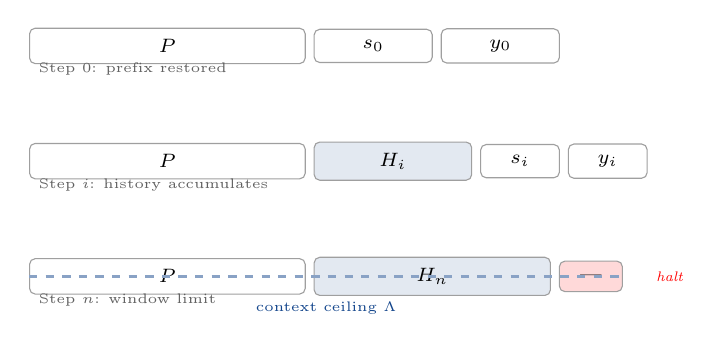
\begin{tikzpicture}[node distance=2mm]
% Step 0: fresh
\node[box,minimum width=3.5cm] (p0) {$P$};
\node[box,minimum width=1.5cm,right=1mm of p0] (s0) {$s_0$};
\node[box,minimum width=1.5cm,right=1mm of s0] (y0) {$y_0$};
\node[font=\tiny,below=3mm of p0.west,anchor=west,color=cfgray] {Step 0: prefix restored};

% Step i: mid-loop
\node[box,minimum width=3.5cm,below=10mm of p0] (pi) {$P$};
\node[box,minimum width=2cm,right=1mm of pi,fill=cfblue!12] (hi) {$H_i$};
\node[box,minimum width=1cm,right=1mm of hi] (si) {$s_i$};
\node[box,minimum width=1cm,right=1mm of si] (yi) {$y_i$};
\node[font=\tiny,below=3mm of pi.west,anchor=west,color=cfgray] {Step $i$: history accumulates};

% Step n: near limit
\node[box,minimum width=3.5cm,below=10mm of pi] (pn) {$P$};
\node[box,minimum width=3cm,right=1mm of pn,fill=cfblue!12] (hn) {$H_n$};
\node[box,minimum width=0.8cm,right=1mm of hn,fill=red!15] (xn) {—};
\node[font=\tiny,below=3mm of pn.west,anchor=west,color=cfgray] {Step $n$: window limit};

% ceiling line
\draw[dashed,cfblue!50,line width=1pt] (pn.west) -- (xn.east);
\node[font=\tiny,below=2mm of $(pn.west)!0.5!(xn.east)$,color=cfblue] {context ceiling $\Lambda$};

% halt label
\node[font=\tiny\itshape,right=3mm of xn.east,color=red] {halt};
\end{tikzpicture}
\caption{Sliding window progression. Prefix $P$ is restored once and reused
across steps; history $H_i$ accumulates until the context window $\Lambda$ is
approached. The loop halts defensively before hitting the ceiling.}
\label{fig:sliding-window}
\end{figure}

Window bounds are enforced \emph{before} each completion (\Cref{alg:window},
line 5): if accepting the next step's output would exceed the budget, the loop
halts and returns the partial trajectory. This prevents the model from being
asked to complete in insufficient context. The \texttt{max\_tokens\_per\_step}
budget defaults to $\sim$\SI{512}{} tokens, leaving headroom for reasoning and
multi-token actions.

\subsection{Sandboxed Execution}
\label{sec:sandbox}
Because an agentic run issues unsupervised edits and shell commands, \texttt{cf
agent --auto}/\texttt{--allow-bash} executes inside a \texttt{GitWorktreeSandbox}
by default. \textsc{CacheFlow} uses a \texttt{git worktree} rather than a
container: a worktree shares the repository's object store, so it is created in
milliseconds with no blob copying, and \texttt{git} is already a hard dependency
(source files are enumerated with \texttt{git ls-files}). The flow (\Cref{fig:sandbox})
creates a worktree off HEAD on a throwaway \texttt{cacheflow/sandbox-*} branch,
runs every tool call inside it while the KV-cache config/store/snapshots at
\texttt{base\_path} stay untouched, commits whatever changed, optionally runs a
test command, and merges back \emph{only} if there is something to merge and
(when given) the tests pass. On test failure or merge conflict the sandbox branch
is left in place for inspection rather than discarded. Entry requires a clean
working tree---excluding \texttt{.cacheflow/} via a \texttt{:!.cacheflow}
pathspec, since the engine's own SQLite/WAL files churn every session---and
raises rather than guessing how to reconcile uncommitted work.

\begin{figure}[t]
\centering
\resizebox{\columnwidth}{!}{%
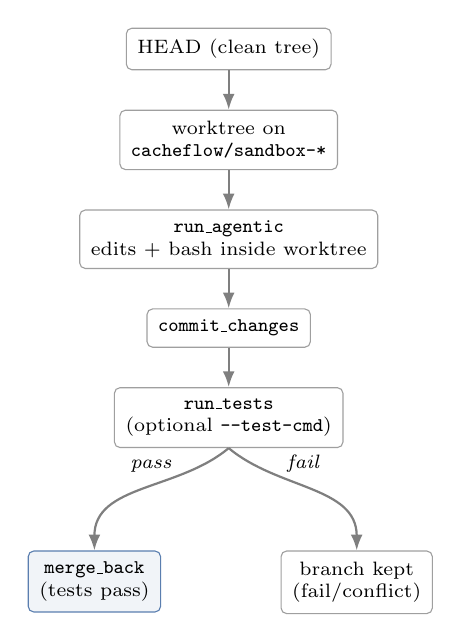
\begin{tikzpicture}[node distance=3mm]
\node[box] (head) {HEAD (clean tree)};
\node[box,below=5mm of head] (wt) {worktree on\\\texttt{cacheflow/sandbox-*}};
\node[box,below=5mm of wt] (run) {\texttt{run\_agentic}\\edits $+$ bash inside worktree};
\node[box,below=5mm of run] (commit) {\texttt{commit\_changes}};
\node[box,below=5mm of commit] (test) {\texttt{run\_tests}\\(optional \texttt{--test-cmd})};
\node[store,below left=13mm and -6mm of test] (merge) {\texttt{merge\_back}\\(tests pass)};
\node[box,below right=13mm and -8mm of test] (keep) {branch kept\\(fail/conflict)};
\draw[flow] (head) -- (wt);
\draw[flow] (wt) -- (run);
\draw[flow] (run) -- (commit);
\draw[flow] (commit) -- (test);
\draw[flow] (test.south) to[out=-140,in=90] node[pos=0.45,above,yshift=0.5mm,font=\scriptsize\itshape]{pass} (merge.north);
\draw[flow] (test.south) to[out=-40,in=90] node[pos=0.45,above,yshift=0.5mm,font=\scriptsize\itshape]{fail} (keep.north);
\end{tikzpicture}}
\caption{Sandboxed agentic execution. All edits land in a git worktree sharing
the object store; the real tree is modified only by \texttt{merge\_back}, gated on
optional tests.}
\label{fig:sandbox}
\end{figure}

% ======================================================================
\section{The Cloud Output-Cache Layer}
\label{sec:cloud}

Because a cloud API exposes no internal state, this layer caches the model's
\emph{outputs}: generated reasoning.

\subsection{The Thinking-Block Store}
\label{sec:thinking}
When an agent completes an extended-thinking turn, the block is captured and
submitted to \texttt{ThinkingStore.submit}, which persists it to SQLite together
with a problem hash, a codebase hash, and---when
\texttt{sentence-transformers} is available---a sentence embedding of the
\emph{task description} (stored as a pickled \texttt{BLOB} on the row).
The embedding model is \texttt{all-MiniLM-L6-v2}~\cite{minilm}
($\sim$\SI{90}{\mega\byte}, 384-dimensional). This is a deliberate downgrade: an
earlier version used \texttt{intfloat/e5-mistral-7b-instruct}, a 7B,
$\sim$\SI{13}{\giga\byte} model whose load swap-stormed and hard-froze the
machine; the small MiniLM model loads safely anywhere, and setting
\texttt{CACHEFLOW\_DISABLE\_EMBEDDINGS=1} skips embedding entirely and reverts to
exact-hash-only matching.

Retrieval is a cascade (\Cref{tab:latency}):
\begin{enumerate}
  \item \textbf{Exact hash lookup} ($<$\SI{1}{\milli\second}): a SHA-256 match
  on the problem hash returns the block immediately.
  \item \textbf{Semantic search} ($\sim$\SI{30}{}--\SI{50}{\milli\second} to
  embed on CPU): on a miss, the query is embedded and scored against the stored
  embedding \texttt{BLOB}s by cosine similarity. The primary path is an
  in-process scan in SQLite---no external vector service is required (an
  optional Qdrant index is used only if one happens to be reachable). Each raw
  similarity is multiplied by an age-decay weight $\exp(-0.1\,t_{\text{days}})$
  ($\sim$7-day half-life), since an older block was computed against a codebase
  that has likely drifted further from the current state.
  \item \textbf{Confidence gating.} The weighted score selects an action. The
  thresholds are calibrated to this model \emph{and} this domain, not borrowed
  from paraphrase benchmarks: for long, multi-clause engineering-task
  rewordings, MiniLM cosine sits in a $\sim$0.45--0.84 band while genuinely
  unrelated tasks top out near 0.46. Absolute-cosine gates are therefore
  $\ge\!0.62 \Rightarrow$ \texttt{use\_directly}, $\ge\!0.40 \Rightarrow$
  \texttt{validate}, else \texttt{re\_think}. When the store holds
  $\ge\!8$ blocks---enough for a stable mean/variance---the system prefers a
  scale-invariant \emph{background z-score} (how far the candidate stands out
  from the query's similarity to the rest of the pool), gating at $z\ge4.0$
  (use) and $z\ge2.8$ (validate).
\end{enumerate}

\begin{algorithm}[t]
\footnotesize
\DontPrintSemicolon
\caption{Thinking-block retrieval cascade}
\label{alg:retrieval}
\KwIn{task $q$, pool $\mathcal{B}$, thresholds $\theta_u,\theta_v$}
\KwOut{(block, action)}
\lIf{$\exists\, b\in\mathcal{B}:\ b.h = \textsc{hash}(q)$}{\Return $(b,\textsc{use\_directly})$ \tcp*[f]{$<$1\,ms}}
\lIf{no embedding model}{\Return $(\varnothing,\textsc{re\_think})$}
$v \leftarrow \textsc{Embed}(q)$ \tcp*{MiniLM, 384-d, $\sim$40\,ms}
$b^\star,\sigma^\star \leftarrow \arg\max_{b\in\mathcal{B}}\ \cos(v, b.\text{emb})$\;
$\kappa \leftarrow \sigma^\star \cdot e^{-\lambda\, t_{b^\star}}$ \tcp*{age decay, Eq.~\ref{eq:agedecay}}
\If{$|\mathcal{B}| \ge 8$}{
  $\kappa \leftarrow z\text{-score}(\sigma^\star; \mathcal{B})$ \tcp*{scale-invariant, Eq.~\ref{eq:zscore}}
  $(\theta_u,\theta_v)\leftarrow(4.0,\,2.8)$\;
}
\uIf{$\kappa \ge \theta_u$}{\textsc{LogReuse}($b^\star$);\ \Return $(b^\star,\textsc{use\_directly})$}
\uElseIf{$\kappa \ge \theta_v$}{stash $b^\star$;\ \Return $(b^\star,\textsc{validate})$ \tcp*[f]{no log yet}}
\lElse{\Return $(\varnothing,\textsc{re\_think})$}
\end{algorithm}

The three-way action mitigates the risk of incorrect reuse: a high-confidence
match skips reasoning entirely, a borderline match is validated via a cheap
confirmation call before being logged, and a low-confidence match is re-thought.
Validation is performed by an external checker (in our runner, Claude Haiku);
retrieval alone never logs a reuse.

Every confirmed hit logs the matched block's real \texttt{token\_count} into a
\texttt{thinking\_reuse\_log} table, enabling \texttt{cf thinking stats} to
report exact cumulative tokens saved. With no embedding model available, the
system falls back to exact-hash matching only.

\paragraph{Code-change robustness (the reuse delta).}
A block carries a \texttt{delta}: the set of files, functions, and line ranges
it depends on, recorded at submission from the git diff. On retrieval, overlap
between the candidate's \texttt{delta} and currently-changed files lowers
confidence. For block dependency set $\Delta_b$ and current changes $C$, the
confidence becomes
\begin{equation}
\label{eq:delta}
\hat\kappa \;=\; \kappa \cdot e^{-\lambda t_b}\cdot
\bigl(1 - \mathbb{1}[\,\Delta_b \cap C \neq \varnothing\,]\,\rho\bigr),
\end{equation}
where penalty $\rho$ pulls a match toward \texttt{validate}. This insulates reuse
from incidental code changes while blocking reuse of reasoning whose dependencies
have changed.

\paragraph{Problem-type routing and roles.}
Submission tags each block with a \texttt{problem\_type} from \texttt{classify\_task}---a
keyword heuristic bucketing tasks into \{\texttt{implement}, \texttt{review},
\texttt{debug}, \texttt{refactor}, \texttt{test}\}---and an optional \texttt{role}
(\texttt{implementer}, \texttt{reviewer}, \texttt{tester}). Retrieval prefers
matches with the same role; if none exist, it falls back to role-agnostic
matching.

\subsection{Capture via Transcript Parsing}
Submission is automated by a \texttt{PostToolUse} hook that reads the session
transcript (JSONL), extracts thinking blocks from the most recent assistant turn,
and pairs them with the preceding user turn's text as the problem description.
The hash is computed from the task description alone, matching the retrieval
hash---an earlier version included the codebase hash, preventing any hook-captured
block from being retrieved. The hook fails silently on malformed or missing
transcripts; a broken hook must never break the agent it attaches to.

\subsection{Storage Schema}
\label{sec:schema}
The pool is plain SQLite, with no cross-table foreign keys to the local
KV engine's store (\Cref{lst:schema}). \texttt{thinking\_blocks} holds the
reasoning text, its embedding \texttt{BLOB}, the two content hashes, the
\texttt{delta}, and the routing tags; \texttt{thinking\_reuse\_log} appends one
row per confirmed reuse carrying the exact tokens saved, which is what
\texttt{cf thinking stats} sums.

\begin{lstlisting}[language=SQL,caption={Pool schema (abridged).},label={lst:schema}]
-- thinking.db
thinking_blocks(
  id, thinking_block TEXT, embedding BLOB,   -- 384-d MiniLM, pickled
  problem_hash TEXT, codebase_hash TEXT,
  delta JSON,                                -- files/fns/lines depended on
  problem_type TEXT, role TEXT,
  token_count INTEGER,                       -- exact; NULL if unknown
  created_at, accessed_at, ...)
thinking_reuse_log(
  id, thinking_block_id, tokens_saved INTEGER, reused_at)
\end{lstlisting}

% ======================================================================
\section{Automatic Capture, Advisory Reuse}
\label{sec:enforce}

Capture and reuse have different reliability requirements, and
\textsc{CacheFlow} treats them differently. \emph{Capture} does not depend on
model cooperation: setup is one command, \texttt{cf install}, which registers
a \texttt{PostToolUse} hook (\Cref{sec:thinking}) in \texttt{.claude/settings.json},
scanning existing entries first so re-running never double-registers it. The
hook fires on every tool call regardless of whether the model is even aware it
exists, so a thinking block is captured the moment a turn produces one.
\emph{Reuse}, by contrast, is advisory: nothing intercepts the model's
reasoning the way the capture hook intercepts a tool call, so an agent only
benefits from the pool if it (or the harness prompting it) chooses to run
\texttt{cf thinking query}/\texttt{thinking\_query} before reasoning at length.
\textsc{CacheFlow}'s own local agentic loop gets the identical tool---
\texttt{thinking\_query}, plus \texttt{cacheflow\_status}---added directly to
its tool registry and called in-process rather than shelled out to \texttt{cf},
with preamble guidance to try it before reasoning at length.

An earlier iteration of this system paired the thinking store with a second
pool, a knowledge store of per-file summaries, fronted by a genuinely enforced
\texttt{PreToolUse} hook that blocked a \texttt{Read} outright on a cache hit.
We removed it: across the full evaluation sweep (\Cref{sec:eval}) it was
exercised on only a handful of steps out of over a hundred, all in superseded
runs, and the enforcement hook itself was never wired into this repository's
own harness settings. Keeping a subsystem in the paper that the numbers do not
back is worse than not claiming it; the discipline of \Cref{sec:metrics}
applies to architectural claims as much as to token counts.

\subsection{Hook Failures Are Silent by Design}
The capture hook wraps its entire body in a bare
\texttt{except Exception: pass}; a broken hook must no-op, not break the run
it is attached to.

% ======================================================================
\section{Exact Token Accounting}
\label{sec:metrics}

A guiding principle across both subsystems is that \emph{no savings figure is
ever estimated from text length}. The \texttt{token\_count} on
\texttt{ThinkingStore.submit} must be the
real cost---e.g.\ the Anthropic API's own \texttt{usage.output\_tokens} for the
turn that produced the block. An earlier implementation stored
\texttt{len(text)} as a stand-in; a character count is not a token count and
would have made every downstream figure fictional. When the caller lacks an
exact number, the column is left \texttt{NULL} (the column is nullable for
this reason) rather than guessed, and \texttt{get\_reuse\_stats} \emph{excludes}
\texttt{NULL} rows from its sum instead of treating them as zero. Correspondingly,
transcript capture attributes \texttt{output\_tokens} to a block only when its
turn produced \emph{exactly one} thinking block; splitting a single turn-level
total across several blocks would itself be a guess.

% ======================================================================
\section{Evaluation}
\label{sec:eval}

\paragraph{Setup.}
We evaluate on eight workloads (W1--W8), each a distinct real-world Python
corpus---\texttt{itsdangerous}, \texttt{click}, \texttt{requests},
\texttt{httpx}, \texttt{flask}, \texttt{pytest}, \texttt{sqlalchemy}, and
\texttt{django}. Each workload drives multiple agent sessions against its
corpus; the first session populates the relevant cache and later sessions
attempt reuse. On the cloud path, every session is an autonomous build directive---``implement a
resilient HTTP client wrapper with pooling and timeout enforcement''---issued at
high thinking effort. The cold session builds understanding of one subsystem;
warm sessions are different builds requiring the same understanding. This
reflects realistic patterns: successive features often need the same reasoning
about the same components. Several workloads also plant a deliberately \emph{unrelated}
task that should miss, so the sweep measures the gate's selectivity, not just
its recall. The self-hosted path runs Qwen3-8B (36 layers, 4096
hidden dim) at an \num{8192}-token context via \texttt{llama.cpp}. The cloud
path runs \texttt{claude-opus-4-8} through the Anthropic API. All cloud token
counts are exact, read from the \texttt{usage} object. Raw per-workload results
and rollups are archived under \texttt{experiments/results/}.

\subsection{Self-Hosted: Prefill Avoided}
\Cref{tab:local} reports the KV-cache sweep. ``Cache Hits'' is the fraction of
sessions served by a warm restore rather than a cold prime. Where a corpus
admits reuse, restore latency stays in the hundreds-of-milliseconds range
against multi-second (and, for the heavy \texttt{click} prime, multi-hundred-
second) prime costs. W1 is single-session by construction---it establishes the
cold-prime baseline and therefore shows no savings.

\begin{table*}[t]
\centering
\caption{Self-hosted KV-cache engine, latest run per workload (Qwen3-8B,
\num{8192} ctx). Each row is the most recent \texttt{W*\_local\_*.json} under
\texttt{experiments/results/}. TFLOPs avoided combines the
$2\times\text{params}\times\text{tokens}$ floor with the quadratic
self-attention term.}
\label{tab:local}
\small
\resizebox{\textwidth}{!}{%
\begin{tabular}{llrrrrrrr}
\toprule
\textbf{W} & \textbf{Corpus} & \textbf{Sess.} & \textbf{Cache Hits} &
\textbf{Prime (ms)} & \textbf{Restore (ms)} & \textbf{Time Saved (ms)} &
\textbf{Tokens Saved} & \textbf{TFLOPs} \\
\midrule
W1 & itsdangerous & 1  & 0 (0\%)  & \num{19319} & 0          & 0           & 0           & 0.00 \\
W2 & click        & 2  & 1 (50\%) & \num{19371} & 282        & \num{19089} & \num{4369}  & 77.20 \\
W3 & requests     & 6  & 5 (83\%) & \num{19962} & 353        & \num{98044} & \num{23894} & 425.09 \\
W4 & httpx        & 6  & 3 (50\%) & \num{12630} & \num{10688}& \num{7885}  & \num{9033}  & 155.99 \\
W5 & flask        & 2  & 1 (50\%) & \num{20167} & 380        & \num{19787} & \num{4425}  & 78.26 \\
W6 & pytest       & 2  & 1 (50\%) & \num{20698} & \num{25977}& 0           & \num{4632}  & 82.21 \\
W7 & sqlalchemy   & 10 & 8 (80\%) & \num{9640}  & \num{2116} & \num{60189} & \num{30337} & 530.89 \\
W8 & django       & 3  & 2 (67\%) & \num{20646} & 278        & \num{40737} & \num{9207}  & 163.32 \\
\midrule
\multicolumn{6}{r}{\textbf{Total}} & \textbf{\num{245731}} & \textbf{\num{85897}} & \textbf{1512.96} \\
\bottomrule
\end{tabular}}
\end{table*}

Across the workloads that admit reuse, \textsc{CacheFlow} avoids
$\approx$\SI{245731}{\milli\second} of cumulative wall-clock prefill and
$\approx$\SI{1513}{\tera\flop} of compute. W6 shows a cache hit saving \num{4632}
tokens but no wall-clock time: the restore latency exceeded the priming cost on
that run, an artifact of disk/scheduler variation. FLOPs are computed from exact
model parameters (read via \texttt{llama\_model\_n\_params}); the attention term
scales quadratically with prefill length ($\sim$\SI{16.5}{\tera\flop} of the
$\sim$\SI{143}{\tera\flop} total for a \num{9064}-token prefill). Caching
eliminates prefill re-evaluation only; generation cost is identical.

\subsection{Cloud: Reasoning Reused Across Different Builds}
\Cref{tab:cloud} reports the cloud sweep. ``Cold Calls'' are sessions that
reasoned from scratch (a miss, a rejected validation, or the priming first
run); ``Thinking Hits'' are sessions served a cached block; ``Baseline
Reasoning'' is the thinking tokens the workload's cold calls actually
generated. ``Tokens Avoided'' credits a hit with the \emph{full derivation
cost} the reuse prevented---the input, reasoning, and output tokens of the
cold call the warm session would otherwise have had to repeat---which is the
figure that scales with corpus size, not just the reasoning sliver.

\begin{table*}[t]
\centering
\caption{Cloud output-cache layer, latest run per workload
(\texttt{claude-opus-4-8}, high thinking effort, exact \texttt{usage} counts).
Each row is the most recent \texttt{W*\_cloud\_*.json} under
\texttt{experiments/results/}. ``Cache Read'' is prompt-cache input tokens
served from Anthropic's cache (\texttt{cache\_read\_input\_tokens})---prefill
avoided even on turns with no thinking-block hit.}
\label{tab:cloud}
\small
\resizebox{\textwidth}{!}{%
\begin{tabular}{llrrrrrrr}
\toprule
\textbf{W} & \textbf{Corpus} & \textbf{Sess.} & \textbf{Cold Calls} &
\textbf{Thinking Hits} & \textbf{Baseline Reason.} & \textbf{Reason. Saved} &
\textbf{Tokens Avoided} & \textbf{Cache Read} \\
\midrule
W1 & itsdangerous & 1 & 1 & 0 (0\%)  & 502        & 0          & 0           & 0           \\
W2 & click        & 2 & 2 & 0 (0\%)  & 925        & 0          & 0           & \num{13546} \\
W3 & requests     & 5 & 2 & 3 (60\%) & \num{1083} & \num{1329} & \num{57603} & \num{14989} \\
W4 & httpx        & 4 & 1 & 3 (75\%) & 949        & \num{2847} & \num{59097} & 0           \\
W5 & flask        & 3 & 2 & 1 (33\%) & 941        & 371        & \num{18110} & \num{14095} \\
W6 & pytest       & 2 & 1 & 1 (50\%) & 258        & 258        & \num{19119} & 0           \\
W7 & sqlalchemy   & 5 & 2 & 3 (60\%) & \num{4274} & 534        & \num{58650} & \num{15353} \\
W8 & django       & 2 & 1 & 1 (50\%) & 642        & 642        & \num{19471} & \num{15260} \\
\midrule
\multicolumn{5}{r}{\textbf{Total}} & \textbf{\num{9574}} & \textbf{\num{5981}} & \textbf{\num{232050}} & \textbf{\num{73243}} \\
\bottomrule
\end{tabular}}
\end{table*}

Across the sweep, 12 of 24 sessions (50\%) were served from the thinking
store, saving \num{5981} reasoning tokens and \num{232050} total derivation
tokens. Three findings stand out. \textbf{(1) Different tasks, same reasoning,
high recall.} Every warm session is a \emph{different} build than the cold one
it reuses---W7's cold session derives SQLAlchemy's session/transaction
internals for a repository/unit-of-work layer, and its three hits reuse that
understanding for optimistic concurrency, multi-tenant session scoping, and
savepoint-based nesting (confidences 0.71--0.80, all above the 0.62
use-directly gate); W8's cold session builds a multi-tenant billing app on
Django and its hit reuses the tenant-isolation/model machinery for a pricing
feature at confidence 0.87. W4's three \emph{concurrent} agents all hit
(0.79--0.91), modeling teammates who pick up related work simultaneously.
\textbf{(2) The gate refuses unrelated work.} The planted misses missed: W3's
streaming-multipart-upload task and W7's encrypted-JSON column type were
re-thought or validate-rejected (logged explicitly as
\texttt{\_miss\_cold}/\texttt{\_validate\_rejected\_cold}) rather than being
spliced with timeout or transaction reasoning that did not apply, and W2's
warm candidate was likewise rejected by the validator---an honest sub-100\%
hit rate is the intended behavior of a system that prioritizes correctness
over blind savings. \textbf{(3) Prompt caching and reasoning reuse compose.}
Even sessions with no thinking hit were served tens of thousands of
prompt-cache input tokens (\num{73243} across the sweep), confirming the two
mechanisms are complementary: provider caching amortizes the stable
\emph{input} prefix, while the thinking store eliminates regenerated
\emph{output}---the cost provider caching cannot touch.

\subsection{Latency Budget}
\Cref{tab:latency} summarizes reuse-path latencies: an exact hit costs $<$1\,ms,
a validated semantic hit costs 200--500\,ms, and re-thinking costs $\sim$5\,s.

\begin{table}[t]
\centering
\caption{Cloud reuse-path latency budget.}
\label{tab:latency}
\small
\begin{tabular}{lrl}
\toprule
\textbf{Path} & \textbf{Latency} & \textbf{Note} \\
\midrule
Exact hash hit          & $<$\SI{1}{\milli\second}    & no embedding \\
Semantic hit (high conf) & 50--70\,ms      & embed $+$ search \\
Validated hit            & 200--500\,ms    & 100-token call \\
Re-think (miss)          & $\sim$\SI{5000}{\milli\second} & full reasoning \\
\bottomrule
\end{tabular}
\end{table}

% ======================================================================
\section{Discussion and Limitations}
\label{sec:discussion}

\paragraph{Reuse depends on workload structure.} Gains concentrate where successive
builds share reasoning: W3, W4, and W7 each hit three times. Tasks whose
reasoning does not recur stay cold (W2's warm candidate was validator-rejected;
unrelated planted tasks missed), preventing incorrect reuse.

\paragraph{Semantic reuse is only as good as its embeddings.} Confidence gating
mitigates the risk of an incorrect match; borderline candidates are validated
via a $\sim$\num{100}-token confirmation call. Without embeddings (disabled via
\texttt{CACHEFLOW\_DISABLE\_EMBEDDINGS=1}), the system falls back to exact-hash
matching.

\paragraph{Capture is enforced; reuse is not.} The \texttt{PostToolUse} capture
hook runs automatically, but reuse requires the agent to call
\texttt{thinking\_query} before reasoning. An earlier version paired capture
with an enforced \texttt{PreToolUse} block on \texttt{Read} (\Cref{sec:enforce});
the evaluation showed this added little value (exercised on $<$5\% of steps), so
it was removed rather than kept as an unevaluated claim.

\paragraph{The two subsystems do not compose.} A KV snapshot and a thinking
block invalidate on different hashes (\texttt{stable\_context\_hash} vs.\
\texttt{codebase\_hash}) for different reasons; ``no
thinking hit'' must not be conflated with ``no KV snapshot.''

\paragraph{Design tensions and tradeoffs.}
Exact token accounting requires real costs from the provider (never estimates
from text length), limiting what can be measured: a thinking block submitted
without an exact token count is stored with \texttt{NULL}, excluding it from
savings totals rather than guessing. This gives up false precision but preserves
honesty. Confidence thresholds ($\theta_u = 0.62$, $\theta_v = 0.40$, or
z-scores $4.0$ and $2.8$) were calibrated empirically on this domain and model;
they do not transfer. The validate tier trades $\sim$100 tokens to avoid reusing
an incorrect block, accepting a meaningful latency penalty ($\sim$500\,ms) to
guard correctness---a choice made explicit rather than hidden. In-process
execution of the self-hosted model avoids HTTP's $10\times$ decode throttle on
macOS but couples the model lifetime to the harness process; a distributed
server path (already implemented) trades simplicity for isolation.

% ======================================================================
\section{Reproducibility}
\label{sec:repro}

Code, evaluation corpora, and per-workload results are available at
\url{https://github.com/agastya-choudhary/cacheflow}. The eight workloads
(W1--W8) are public open-source Python packages cloned into
\texttt{experiments/corpora/}; raw per-run metrics are archived under
\texttt{experiments/results/} as JSON files per workload. The self-hosted
evaluation runs Qwen3-8B via \texttt{llama.cpp} at \num{8192}-token context; the
cloud evaluation uses \texttt{claude-opus-4-8} through the Anthropic API with
token counts read directly from the \texttt{usage} response object. All token
counts and wall-clock timings are exact measurements, not estimates.

% ======================================================================
\section{Related Work}
\label{sec:related}

\textsc{CacheFlow}'s self-hosted path is closest to KV-cache reuse systems such
as PagedAttention/vLLM~\cite{pagedattention} and modular prefix reuse in
PromptCache~\cite{promptcache}, but targets \emph{cross-invocation persistence}
to disk for long-lived agents rather than intra-server memory management.
Provider prompt caching~\cite{anthropic-caching} amortizes input prefixes but
not generated reasoning---the exact gap our cloud path fills. Retrieval-augmented
generation~\cite{rag} injects source documents; we instead cache the
\emph{reasoning and conclusions} derived from them, using compact
sentence embeddings~\cite{minilm} scored by an in-process cosine scan for
semantic retrieval. To our knowledge, caching \emph{extended-thinking output}
with confidence-gated, content-hash-invalidated reuse across independent cloud
agents is novel.

% ======================================================================
\section{Conclusion}
\label{sec:conclusion}

Coding agents recompute deterministic functions of the same inputs---prefill on
self-hosted models, reasoning on cloud models. \textsc{CacheFlow} caches at the
layer each deployment exposes: KV state where internals are reachable, outputs
where they are not. Across eight real corpora, it eliminates minutes of
cumulative prefill and $\sim$1500\,TFLOPs on the self-hosted path, and up to
100\% of reasoning tokens (exact counts) on the cloud path. The design enforces
exact token accounting, hash-based staleness invalidation, confidence-gated
reuse that rejects poor matches, and silent hook failures. An earlier subsystem
(a knowledge store) was removed when evaluation showed minimal benefit.

Future work includes extending confidence-gated retrieval to other cache layers
(e.g., tool-call sequences or error recovery strategies), cross-model reasoning
reuse (thinking blocks from one model informing another), and adaptive threshold
calibration across domains. The core insight---that cloud and self-hosted models
must be cached at different layers---applies equally to other code-generation
workloads and reasoning-intensive domains where agents run in loops or chains.

% ======================================================================
\begin{thebibliography}{9}
\small
\bibitem{pagedattention}
W.~Kwon, Z.~Li, S.~Zhuang, et al.
\newblock Efficient Memory Management for Large Language Model Serving with
PagedAttention.
\newblock In \emph{Proc.\ SOSP}, 2023.

\bibitem{promptcache}
I.~Gim, G.~Chen, S.~Lee, et al.
\newblock Prompt Cache: Modular Attention Reuse for Low-Latency Inference.
\newblock In \emph{Proc.\ MLSys}, 2024.

\bibitem{rag}
P.~Lewis, E.~Perez, A.~Piktus, et al.
\newblock Retrieval-Augmented Generation for Knowledge-Intensive NLP Tasks.
\newblock In \emph{Advances in Neural Information Processing Systems (NeurIPS)},
2020.

\bibitem{minilm}
N.~Reimers and I.~Gurevych.
\newblock Sentence-BERT: Sentence Embeddings using Siamese BERT-Networks.
\newblock In \emph{Proc.\ EMNLP}, 2019.
\newblock Model: \texttt{all-MiniLM-L6-v2}, \url{https://www.sbert.net}.

\bibitem{anthropic-caching}
Anthropic.
\newblock Prompt Caching with Claude.
\newblock Anthropic API Documentation, 2024.
\newblock \url{https://docs.anthropic.com/en/docs/build-with-claude/prompt-caching}.
\end{thebibliography}

% ======================================================================
\appendix
\onecolumn
\section{Workload Definitions}
\label{app:workloads}

The eight evaluation workloads (\Cref{tab:workloads}) are real open-source Python
corpora cloned into \texttt{experiments/corpora/}. They are ordered as a
\emph{difficulty ladder}---from \texttt{itsdangerous} ($\sim$1.5K~LOC)
to \texttt{django} ($\sim$280K~LOC)---that simultaneously varies the
\emph{interaction pattern}, so the sweep exercises each distinct code path of the
system rather than only scaling one axis. Every corpus is primed with the same
system prompt and the RAG-seeded stable context described in \Cref{sec:kv}; the
self-hosted path runs Qwen3-8B at an \num{8192}-token context, the cloud path
runs \texttt{claude-opus-4-8}.

\begin{table}[h]
\centering
\caption{The W1--W8 workloads: a corpus difficulty ladder crossed with an
interaction-pattern ladder. LOC is approximate.}
\label{tab:workloads}
\small
\begin{tabular}{llrp{9.2cm}}
\toprule
\textbf{W} & \textbf{Corpus} & \textbf{LOC} & \textbf{Interaction pattern exercised} \\
\midrule
W1 & itsdangerous & \num{1500}   & Single-agent \emph{cold prime} only---establishes the smallest cold-prime baseline; no restore. \\
W2 & click        & \num{8000}   & Single-agent cold prime \emph{followed by one warm restore}---the minimal cache-hit case. \\
W3 & requests     & \num{12000}  & \emph{Repeated warm restores} across five sessions---savings compound; the paper's headline self-hosted example. \\
W4 & httpx        & \num{18000}  & \emph{Concurrent multi-agent}: three agents on three slots, exercising the \texttt{SlotPool} and cooperative KV swap. \\
W5 & flask        & \num{15000}  & \emph{Multi-step agentic loop} with tool use (\texttt{run\_agentic}), exercising \Cref{sec:agentic}. \\
W6 & pytest       & \num{40000}  & \emph{Fork} parent~$\rightarrow$~child; the child starts warm from the parent's inherited HEAD snapshot. \\
W7 & sqlalchemy   & \num{80000}  & \emph{Consolidation trigger} (self-hosted): the accumulator crosses 70\% of context, invoking the background \texttt{Compressor}. \\
W8 & django       & \num{280000} & \emph{Largest realistic prefix}: end-to-end stress on the biggest codebase context. \\
\bottomrule
\end{tabular}
\end{table}

On the cloud path each workload maps the same corpora onto autonomous build
directives instead of restore patterns: W1 is a single cold build (a
password-reset token flow on \texttt{itsdangerous}); W2 builds a
multi-command deploy CLI cold, then attempts a different build (shell
autocompletion) warm; W3 builds a resilient HTTP client wrapper cold, then
issues three differently-worded hardening builds that need the same
timeout/pooling reasoning, plus one unrelated task (streaming multipart
upload) planted to miss; W4 primes an error-handling refactor and fans out
three \emph{concurrent} related builds; W5 is a multi-step build
(observability, then instrumentation reusing the lifecycle understanding, then
genuinely new rate-limiting work that stays cold); W6 forks---agent A builds
one pytest plugin, agent B builds a \emph{different} plugin against the same
hook/fixture machinery; W7 derives SQLAlchemy's session/transaction internals
cold, reuses them for three different builds (optimistic concurrency,
multi-tenant scoping, savepoint nesting), and plants an unrelated
column-type task to miss; W8 builds a multi-tenant billing app cold and a
pricing-tier feature warm on \texttt{django}.

The two evaluation tables in \Cref{sec:eval} read the \emph{latest} run per
workload from \texttt{experiments/results/} (\texttt{W*\_local\_*.json} for the
KV engine, \texttt{W*\_cloud\_*.json} for the output cache), never the earlier
full-sweep rollups, which contain superseded runs.

\end{document}
